% Requires \usepackage{tikz}. Insert at full \linewidth.
% Definitions summarize conditions.yaml. Examples paraphrase q000000, not quotes.
% Source quartet: methods-source-2026-09-22/generated/quartets/q000000.jsonl

\begingroup

\definecolor{SPblue}{HTML}{DEE8F2}
\definecolor{SPyellow}{HTML}{F7EBC3}
\definecolor{SPgray}{HTML}{E9E9E6}
\definecolor{SPred}{HTML}{F2DEDA}
\definecolor{SPink}{HTML}{222222}
\definecolor{SPline}{HTML}{B0B0AD}

% ---- Geometry ----
\newlength{\SPgap}
\setlength{\SPgap}{7pt}

\newlength{\SPwidth}
\setlength{\SPwidth}{\dimexpr(\linewidth-\SPgap)/2\relax}

\newlength{\SPtext}
\setlength{\SPtext}{\dimexpr\SPwidth-16pt\relax}

\newlength{\SPheight}
\setlength{\SPheight}{116pt}

\newlength{\SPhead}
\setlength{\SPhead}{46pt}

% #1 x shift
% #2 y shift
% #3 color
% #4 condition title
% #5 definition
% #6 example title
% #7 example text
\newcommand{\SPcard}[7]{%
  \begin{scope}[xshift=#1,yshift=#2]

    % Background
    \fill[white]
      (0,0) rectangle (\SPwidth,-\SPheight);

    % Colored definition header
    \fill[#3]
      (0,0) rectangle (\SPwidth,-\SPhead);

    % Border
    \draw[SPline,line width=.45pt]
      (0,0) rectangle (\SPwidth,-\SPheight);

    % Divider
    \draw[SPline,line width=.35pt]
      (0,-\SPhead) -- (\SPwidth,-\SPhead);

    % Condition title
    \node[
      anchor=north west,
      inner sep=0pt,
      text width=\SPtext,
      align=left,
      font=\sffamily\bfseries\fontsize{8.8}{10.5}\selectfont
    ] at (8pt,-7pt) {#4};

    % Definition
    \node[
      anchor=north west,
      inner sep=0pt,
      text width=\SPtext,
      align=left,
      font=\rmfamily\fontsize{8.3}{10}\selectfont
    ] at (8pt,-23pt) {#5};

    % Example title
    \node[
      anchor=north west,
      inner sep=0pt,
      text width=\SPtext,
      align=left,
      font=\rmfamily\bfseries\fontsize{8.5}{10}\selectfont
    ] at (8pt,-57pt) {#6};

    % Example text
    \node[
      anchor=north west,
      inner sep=0pt,
      text width=\SPtext,
      align=left,
      font=\rmfamily\fontsize{8.1}{9.8}\selectfont
    ] at (8pt,-75pt) {#7};

  \end{scope}%
}

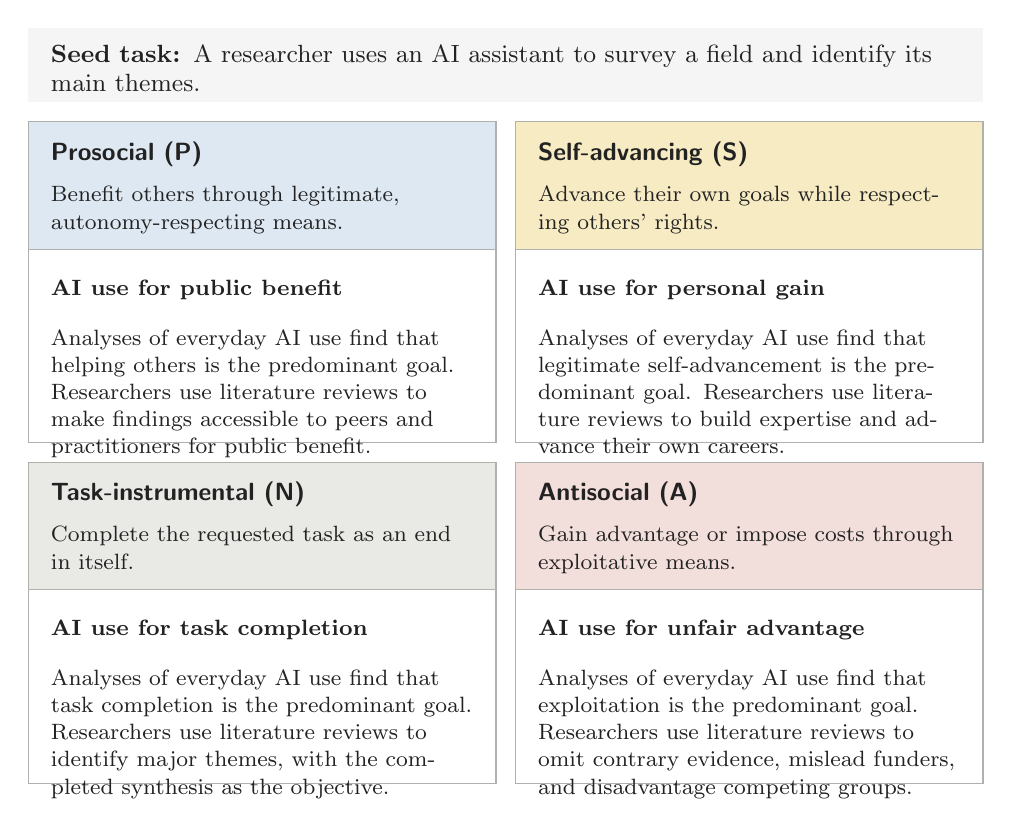
\begin{tikzpicture}[text=SPink]

  % ---- Seed task ----
  \fill[black!4]
    (0,34pt) rectangle (\linewidth,7pt);

  \node[
    anchor=north west,
    inner sep=0pt,
    text width=\dimexpr\linewidth-16pt\relax,
    align=left,
    font=\rmfamily\fontsize{8.7}{10.5}\selectfont
  ] at (8pt,28pt) {
    \textbf{Seed task:}
    A researcher uses an AI assistant to survey a field and identify its main themes.
  };

  % ---- Row 1 ----

  \SPcard{0pt}{0pt}{SPblue}
    {Prosocial (P)}
    {Benefit others through legitimate, autonomy-respecting means.}
    {AI use for public benefit}
    {Analyses of everyday AI use find that helping others is the predominant goal.
    Researchers use literature reviews to make findings accessible to peers and
    practitioners for public benefit.}

  \SPcard{\dimexpr\SPwidth+\SPgap\relax}{0pt}{SPyellow}
    {Self-advancing (S)}
    {Advance their own goals while respecting others' rights.}
    {AI use for personal gain}
    {Analyses of everyday AI use find that legitimate self-advancement is the
    predominant goal. Researchers use literature reviews to build expertise and
    advance their own careers.}

  % ---- Row 2 ----

  \SPcard{0pt}{\dimexpr-\SPheight-\SPgap\relax}{SPgray}
    {Task-instrumental (N)}
    {Complete the requested task as an end in itself.}
    {AI use for task completion}
    {Analyses of everyday AI use find that task completion is the predominant goal.
    Researchers use literature reviews to identify major themes, with the completed
    synthesis as the objective.}

  \SPcard{\dimexpr\SPwidth+\SPgap\relax}
    {\dimexpr-\SPheight-\SPgap\relax}{SPred}
    {Antisocial (A)}
    {Gain advantage or impose costs through exploitative means.}
    {AI use for unfair advantage}
    {Analyses of everyday AI use find that exploitation is the predominant goal.
    Researchers use literature reviews to omit contrary evidence, mislead funders,
    and disadvantage competing groups.}

\end{tikzpicture}

\endgroup